%\documentclass[11pt]{beamer}
\documentclass[11pt,handout,aspectratio=1610]{beamer}

\usepackage[utf8]{inputenc}
\usepackage[T1]{fontenc}
\usepackage[spanish]{babel}
\usepackage{latexsym} 
\usepackage{amsmath}
\usepackage{amsfonts}
\usepackage{amssymb}
\usepackage{esint}
\usepackage{array}
\usepackage{multirow}
\usepackage{xcolor}
\usepackage{graphicx}
\usepackage{tikz}
\tikzset{>=latex}
\usepackage{tikz-3dplot}
\usetikzlibrary{babel}
\usetikzlibrary{calc,patterns,decorations.pathmorphing,decorations.markings}
\usepackage{xcolor}
\usepackage{epstopdf}
\usepackage[nointegrals]{wasysym}
\usepackage{hyperref}
\usepackage{cancel}
\usepackage[font=small,labelfont={small,bf},margin=0.5cm,justification=justified]{caption}
\usepackage[font=small,labelfont={small,bf}]{subcaption}

\usetheme{Berkeley}
\usecolortheme{seahorse}
\uselanguage{Spanish}

\newcommand{\sgn}{\mathop{\text{sgn}}}
\newcommand{\diff}[0]{\text{d}}
\newcommand{\fdiff}[2]{\dfrac{\text{d} #1}{\text{d} #2}}
\newcommand{\pdiff}[2]{\frac{\partial #1}{\partial #2}}
\newcommand{\fddiff}[2]{\frac{\text{d^2} #1}{\text{d} #2^2}}
\newcommand{\grado}[0]{^{\circ}}
\newcommand{\chel}[4]{^{#1}_{#2}\text{#3}^{#4}}
\newcommand{\valmed}[1]{\left\langle #1 \right\rangle}
\newcommand{\E}[1]{\times 10^{#1}}
\newcommand{\ver}[1]{\hat{\vec{#1}}}
\newcommand{\vecg}[1]{\boldsymbol{#1}}
\newcommand{\iu}{\text{i}}
\newcommand{\norm}[1]{\left\vert\left\vert #1 \right\vert\right\vert}
\newcommand{\abs}[1]{\left\vert #1 \right\vert}
\newcommand{\tens}[1]{\mathbb{#1}}
\newcommand{\rr}{\mathbb{R}}
\newcommand{\logoUNAHUR}{
\includegraphics[scale=0.15]{/home/shluna/Proyectos/Clases_Fisica_III/imgs/logo-universidad-nacional-de-hurlingham_preview_rev_1.png}}
\newcommand{\vs}{\vspace{11pt}}
\newcommand{\un}[1]{\text{#1}}

\tikzstyle{dark water}=[draw=mydarkblue,top color=darkwatercol,bottom color=darkwatercol!80!black,shading angle=5]
\tikzstyle{force}=[->,myred,very thick,line cap=round]
\colorlet{myred}{red!65!black}
\colorlet{darkwatercol}{blue!80!cyan!20!white}
\colorlet{mydarkblue}{blue!50!black}

\title{Introducción a la teoría de la elasticidad}
\subtitle{Unidad 3}
\author{Física III}
\institute{Instituto de Tecnología e Ingeniería \\ \vspace{0.25cm} Universidad Nacional de Hurlingham}
\date{ }
\logo{\logoUNAHUR}

\AtBeginSection[]{
  \begin{frame}
  \vfill
  \centering
  \begin{beamercolorbox}[sep=8pt,center,shadow=true,rounded=true]{title}
    \usebeamerfont{title}\insertsectionhead\par%
  \end{beamercolorbox}
  \vfill
  \end{frame}
}

\tdplotsetmaincoords{70}{110}

\begin{document}

\frame{\titlepage}

\begin{frame}{En esta clase veremos:}
    \tableofcontents
\end{frame}

\section{Introducción}

\begin{frame}{Introducción}

    Cuando estudiamos el cuerpo rígido, lo definimos como un sistema de partículas indeformable. Sin embargo, la experiencia nos muestra que todos los cuerpos se deforman en mayor o menor medida cuando se aplican fuerzas sobre ellos.

    \vs

    El propósito de esta unidad es estudiar los aspectos básicos de la denominada \emph{Teoría de la elasticidad:}

    \begin{block}{Teoría de la elasticidad}
        Puede decirse que la elasticidad es la rama de la Física que se ocupa de estudiar la deformación de los cuerpos.
    \end{block}

    A continuación, vamos a comenzar el estudio de la elasticidad definiendo la deformación.

\end{frame}

\section{Deformación}

\begin{frame}{Deformación}

    Cuando estudiamos el movimiento del cuerpo rígido, lo definimos como un sistema de partículas cuyas distancias relativas son constantes: $$ \ell_{ij} = \norm{\vec{r}_i - \vec{r}_j} $$ donde $\ell_{ij}$ es la distancia entre las partículas $i$ y $j$ que se encuentran en los puntos $\vec{r}_i$ y $\vec{r}_j$, respectivamente. 

    \vs 

    %Por supuesto, si esta condición es válida para cualquier par de puntos del cuerpo rígido, en particular lo es para el punto $i$ y el origen de un sistema de referencia que se encuentra dentro del cuerpo y que se mueve solidariamente junto con este y, por lo tanto: $$ \ell_i = \norm{\vec{r}_i} $$ donde ahora $\ell_i$ es la distancia del punto $i$ al origen de dicho sistema de referencia.

    Tal como su nombre lo indica, la deformación implica un cambio o una variación de la forma de un cuerpo.

\end{frame}

\begin{frame}{Deformación}

    Existen diversos tipos de deformación, según la manera en que se apliquen las fuerzas.

    \begin{figure}
        \centering
        \begin{subfigure}{0.3\textwidth}
            \centering
            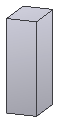
\includegraphics{../figs/mechanics_stress-1.pdf}
            \caption{Sin deformar.}
        \end{subfigure}
        ~
        \begin{subfigure}{0.3\textwidth}
            \centering
            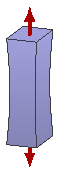
\includegraphics{../figs/mechanics_stress-2.pdf}
            \caption{Tracción.}
        \end{subfigure}
        ~
        \begin{subfigure}{0.3\textwidth}
            \centering
            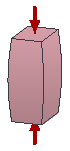
\includegraphics{../figs/mechanics_stress-3.pdf}
            \caption{Compresión.}
        \end{subfigure} \\
        \begin{subfigure}{0.3\textwidth}
            \centering
            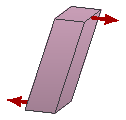
\includegraphics{../figs/mechanics_stress-6.pdf}
            \caption{Corte o cizalladura.}
        \end{subfigure}
        ~
        \begin{subfigure}{0.3\textwidth}
            \centering
            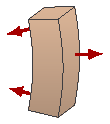
\includegraphics{../figs/mechanics_stress-4.pdf}
            \caption{Flexión.}
        \end{subfigure}
        ~
        \begin{subfigure}{0.3\textwidth}
            \centering
            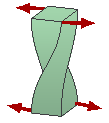
\includegraphics{../figs/mechanics_stress-5.pdf}
            \caption{Torsión.}
        \end{subfigure}
        \caption{Tipos de deformación.}
    \end{figure}

    
\end{frame}

\begin{frame}{Deformación}

    Además de las anteriormente consideradas, existe también la deformación debida a la presión hidrostática.

    \begin{figure}
        \centering
        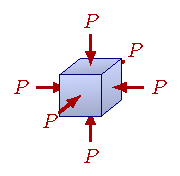
\includegraphics{../figs/fluid_dynamics_pressure-2.pdf}
    \end{figure}

    
\end{frame}

\begin{frame}{Deformación unitaria}

    En esta unidad vamos a estudiar qué ocurre cuando relajamos esta condición. Para ello, debemos primero ver cómo se describe matemáticamente la deformación.

    \vs

    Consideremos, en primer lugar, una barra de longitud $L$, la cual se somete a una fuerza $\vec{F}$, de tracción o de compresión, y que, como consecuencia experimenta un cambio de longitud $\Delta L$.

    \begin{columns}
        \begin{column}{0.5\textwidth}
            \begin{figure}
                \centering
                \begin{subfigure}{\textwidth}
                    \centering
                    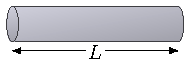
\includegraphics{../figs/mechanics_stress-7.pdf}
                \end{subfigure}
                \\
                \begin{subfigure}{\textwidth}
                    \centering
                    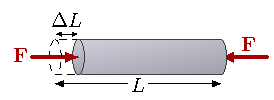
\includegraphics{../figs/mechanics_stress-8.pdf}
                \end{subfigure}
                \\
                \begin{subfigure}{\textwidth}
                    \centering
                    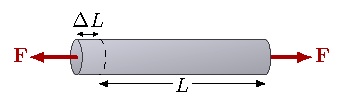
\includegraphics{../figs/mechanics_stress-9.pdf}
                \end{subfigure}
            \end{figure}
        \end{column}
        \begin{column}{0.5\textwidth}
            Definimos la deformación unitaria por tracción o por compresión ($\varepsilon$) como el cambio de longitud por unidad de longitud: $$ \varepsilon = \frac{\Delta L}{L} $$
        \end{column}
    \end{columns}

\end{frame}

\begin{frame}{Deformación unitaria}

    La deformación por corte o cizalladura se origina cuando una fuerza se aplica en dirección paralela a una de las caras del cuerpo.

    \begin{columns}
        \begin{column}{0.5\textwidth}
            \begin{figure}
                \centering
                \begin{subfigure}{\textwidth}
                    \centering
                    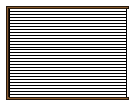
\includegraphics{../figs/mechanics_stress_strain-1.pdf}
                \end{subfigure}
                \\
                \begin{subfigure}{\textwidth}
                    \centering
                    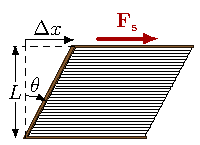
\includegraphics{../figs/mechanics_stress_strain-2.pdf}
                \end{subfigure}
            \end{figure}
        \end{column}
        \begin{column}{0.5\textwidth}
            En este caso, la deformación unitaria por corte o cizalladura se define como el desplazamiento en la dirección de la fuerza por unidad de longitud en la dirección perpendicular a la misma: $$ \varepsilon = \frac{\Delta x}{L} = \tan \theta \approx \theta $$
        \end{column}
    \end{columns}

\end{frame}

\begin{frame}{Deformación unitaria}

    Por último, vamos a considerar la deformación debida a la presión hidrostática, la cual genera una variación del volumen del cuerpo, más específicamente una \emph{disminución}, puesto que esta presión se deba a fuerzas perpendiculares a todas las caras del cuerpo que tienden a comprimir al cuerpo.

    \begin{columns}
        \begin{column}{0.5\textwidth}
            \begin{figure}
                \centering
                \begin{subfigure}{\textwidth}
                    \centering
                    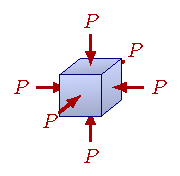
\includegraphics{../figs/fluid_dynamics_pressure-2.pdf}
                \end{subfigure}
            \end{figure}
        \end{column}
        \begin{column}{0.5\textwidth}
            Así, la deformación unitaria por presión hidrostática se define como el cambio de volumen por unidad de unidad de volumen: $$ \varepsilon = \frac{\Delta V}{V} $$
        \end{column}
    \end{columns}

\end{frame}

\begin{frame}{Tensor de deformación}

    Si bien es útil comenzar el estudio de la deformación de un cuerpo viendo cada tipo de deformación por separado, la realidad es que un sólido siempre está sometido a diversas fuerzas que lo deformas en varias direcciones simultáneamente. Es por este motivo que resulta necesaria una descripción más general de la deformación.

    \vs 

    Consideremos dos puntos cualesquiera, $i$ y $j$ de un sólido.

    \begin{columns}
        \begin{column}{0.45\textwidth}
            
        \end{column}
        \begin{column}{0.45\textwidth}
            
        \end{column}
    \end{columns}

\end{frame}

\section{Tensión y fuerzas corporales}

\begin{frame}{Tensión o esfuerzo}

    Como vimos anteriormente, todos los tipos de deformaciones están por supuesto asociadas a alguna fuerza aplicada al cuerpo. Ahora bien, hasta ahora representábamos las fuerzas mediante un vector que tiene un punto de aplicación.

    \vs

    Sin embargo, en términos más estrictos las fuerzas se ejercen mediante el contacto entre dos cuerpos. Este contacto ocurre abarcando cierta área de cada uno de los cuerpos, la cual se denomina superficie de contacto. Así, la fuerza aplicada por un cuerpo sobre otro es en realidad la resultante de las fuerzas distribuidas más o menos uniformemente sobre el área de contacto.

    \vs 

    Asimismo, si se considera una cierta área dentro del cuerpo, la fuerza aplicada sobre éste se distribuye casi uniformemente sobre dicha área.

\end{frame}

\begin{frame}{Tensión o esfuerzo}

    \begin{columns}
        \begin{column}{0.4\textwidth}
            \begin{figure}
                \centering
                \begin{subfigure}{\textwidth}
                    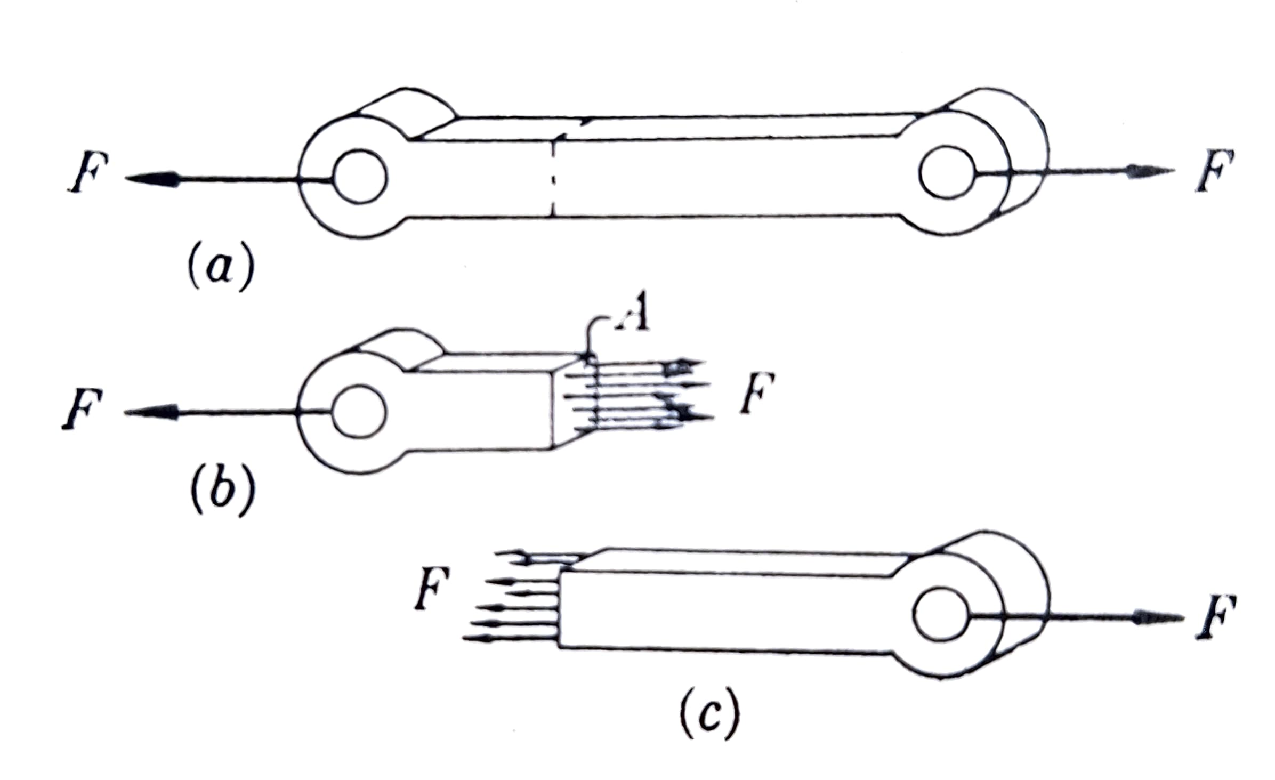
\includegraphics[width=\textwidth]{../figs/tracción.pdf}
                    \caption{Tracción}
                \end{subfigure}
                \\
                \begin{subfigure}{\textwidth}
                    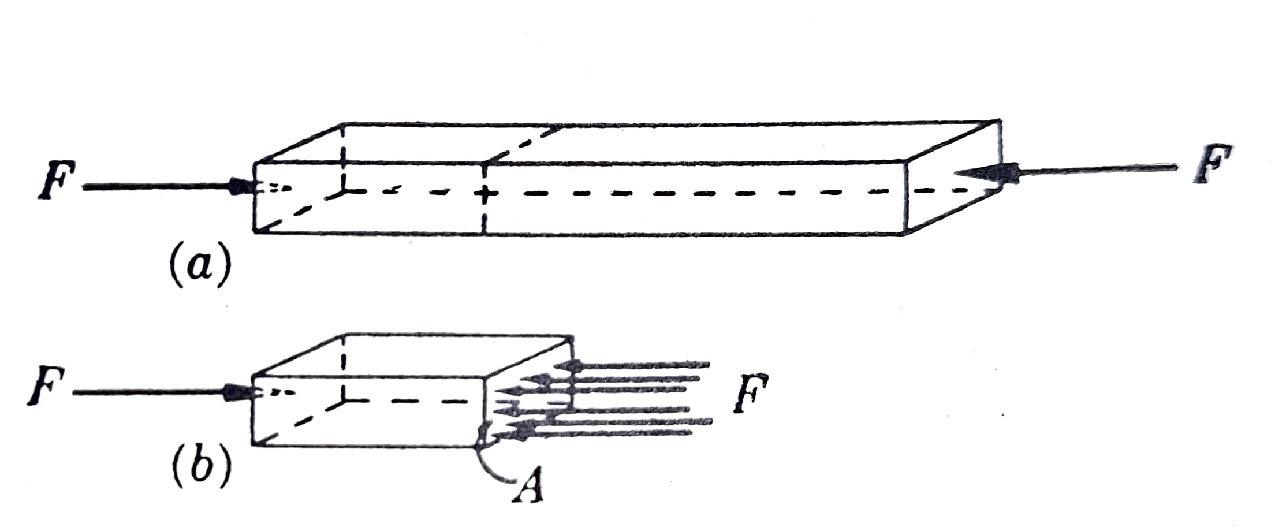
\includegraphics[width=\textwidth]{../figs/compresion.pdf}
                    \caption{Compresión}
                \end{subfigure}
            \end{figure}
        \end{column}
        \begin{column}{0.6\textwidth}
            Si consideramos una barra, a la cual se le aplica una fuerza de tracción o de compresión, y hacemos un corte transversal a una distancia suficiente de donde se aplica la fuerza, tal como se ve en la figura esa fuerza se distribuye por toda esa superficie. En este caso, la fuerza aplicada produce una deformación por compresión o por tracción.

            \vs

            Si se asume que la fuerza aplicada $\vec{F}$ se distribuye uniformemente sobre la superficie transversal de área $A$, definimos la tensión (o el esfuerzo), $\sigma$ como la razón de la fuerza aplicada al área sobre la que se distribuye: $$ \sigma = \frac{F}{A} $$
        \end{column}
    \end{columns}

\end{frame}

\begin{frame}{Tensión o esfuerzo}

    \begin{columns}
        \begin{column}{0.4\textwidth}
            Consideremos ahora una fuerza que se ejerce en dirección paralela a una de las superficies del cuerpo, tal como muestra la figura. Esta fuerza produce una deformación de corte o cizalladura.
        \end{column}
        \begin{column}{0.4\textwidth}
            En este caso, la tensión también se define como la fuerza dividida por el área de la suoerficie sobre la cual se distribuye: $$ \sigma = \frac{F}{A} $$
        \end{column}
    \end{columns}

    \begin{figure}
        \centering
        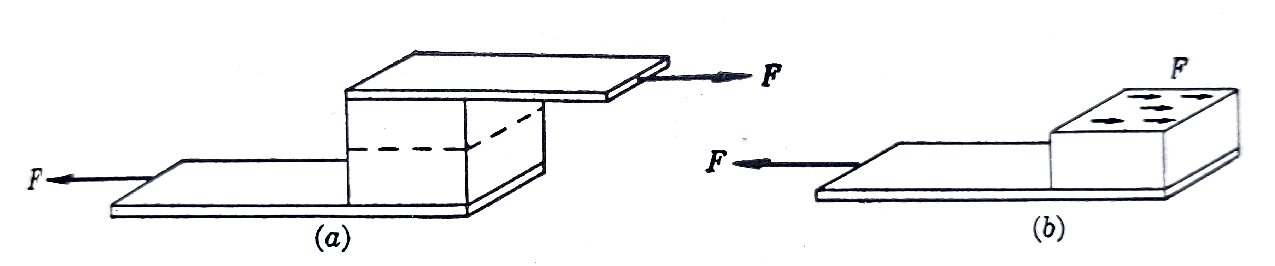
\includegraphics[width=\textwidth]{../figs/cortante.pdf}
        \caption{Corte.}
    \end{figure}

\end{frame}

\begin{frame}{Tensión o esfuerzo}

    \begin{columns}
        \begin{column}{0.4\textwidth}
            \begin{figure}
                \centering
                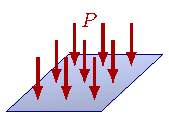
\includegraphics{../figs/fluid_dynamics_pressure-1.pdf}
            \end{figure}
        \end{column}
        \begin{column}{0.4\textwidth}
            De la misma forma se define la tensión o el esfuerzo debido a la presión hidrostática, esto es la fuerza aplicada sobre un área dada del cuerpo: $$ \sigma = \frac{F}{A} = P$$
        \end{column}
    \end{columns}

\end{frame}

\begin{frame}{Fuerzas corporales o de volumen}
    
    A diferencia de las tensiones, las fuerzas coroporales o de volumen son aquellas que actúan en todo el volumen del cuerpo. Tal es el caso de la fuerza de atracción gravitatoria, a través del campo gravitatorio, o la fuerza de interacción eléctrica, a través de un campo eléctrico.

    \vs

    En el caso particular de la fuerza de atracción gravitatoria, podemos considerar el peso de un elemento de masa ($\diff{m}$) del cuerpo. El peso de este elemento de masa es $ \diff \vec{F}_\text{g} = \vec{g} \, \diff{m} $. El diferencial de masa puede escribirse como $\diff{m} = \rho \, \diff{V}$, donde $\rho$ es la densidad y $\diff{V}$ es el volumen del elemento de masa. Entonces: $$ \diff \vec{F}_\text{g} = \vec{g} \, \rho \, \diff{V} $$ Así, el factor $\rho \, \vec{g}$ puede identificarse con la fuerza por unidad de volumen, también conocido como peso específico: $$\vec{f}_\text{g} = \fdiff{\vec{F}_\text{g}}{V} = \rho \, \vec{g} $$

\end{frame}

\begin{frame}{Fuerzas corporales o de volumen}
    
    En términos generales, cualquier fuerza corporal o de volumen puede representarse como una fuerza por unidad de volumen: $$\vec{f} = \rho \, \vec{a}$$ donde $\rho$ es la densidad del elemento de masa del cuerpo y $\vec{a}$ es la aceleración impresa sobre dicho elemento por la fuerza $\vec{f}$.

    \vs

    Cabe destacar que $\vec{f}$ representa la fuerza por unidad de volumen del cuerpo, esto es, la fuerza sobre un elemento de volumen que puede deberse a una causa externa, como se mencionó anteriormente, pero también a las llamadas \emph{tensiones internas}, es decir a las fuerzas que se ejercen entre sí los elementos de volumen adyancentes.

    \vs

    Por supuesto, la fuerza por unidad de volumen tiene unidades de fuerza sobre unidad de volumen. En el caso del SI: $$ \left[\vec{f}\right] = \frac{\un{N}}{\un{m}^3} $$

\end{frame}

\section{Ecuaciones constitutivas y módulos elásticos.}

\begin{frame}{Ecuaciones constitutivas}

    En términos generales, se denomina ecuación constitutiva a la relación entre el esfuerzo y la deformación correspondiente. La forma funcional de cada relación se la conoce como \emph{modelo reológico}.

    \vs 

    \begin{columns}
        \begin{column}{0.4\textwidth}
            \begin{figure}
                \centering
                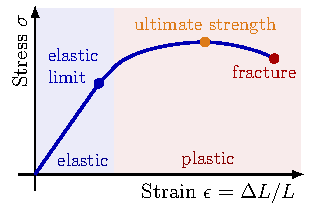
\includegraphics[width=\textwidth]{../figs/mechanics_stress-10.pdf}
            \end{figure}            
        \end{column}
        \begin{column}{0.6\textwidth}
            Dentro de cierto límite, existe una relación lineal entre el esfuerzo y la deformación, esto es $$ \sigma \propto \varepsilon $$ Esto significa que al retirar el esfuerzo aplicado al cuerpo, este recupera totalmente su forma. Para tensiones o deformaciones menores a las definidas por el límite elástico, se dice que el comportamiento del cuerpo es \emph{elástico}.
        \end{column}
    \end{columns}

    \vs

    Tal como se puede apreciar en la Figura, esta relación lineal es válida hasta el denominado \emph{limite elástico}, el cual divide las zonas entre el comportamiento elástico y el comportamiento plástico.

\end{frame}

\begin{frame}{Módulos elásticos}

    A fin de convertir la proporcionalidad en una igualdad, se debe incluir una constante de proporcionalidad. Dicha constante depende del tipo de esfuerzo y de la deformación correspondiente.

    \begin{itemize}
        \item Para el caso de los esfuerzos y las deformaciones de tracción o de compresión, la constante de proporcionalidad se conoce como \emph{módulo de Young} ($E$): $$ E = \frac{\Delta F/A}{\Delta L /L} = \frac{L}{A} \frac{\Delta F}{\Delta L} $$
        \item Cuando se trate de esfuerzos y deformaciones de corte, la constante de proporcionalidad se denomina \emph{módulo de rigidez} ($G$): $$ G = \frac{\Delta F/A}{\Delta x / L} = \frac{L}{A} \frac{\Delta F}{\Delta x}$$
        \item Por último, el \emph{módulo de compresibilidad} ($B$) es la constante que relaciona la deformación por presión hidrostática con la tensión correspondiente: $$ B = - \frac{\Delta P}{\Delta V / V} = - V \frac{\Delta P}{\Delta V} $$
    \end{itemize}

\end{frame}

\begin{frame}{Módulos elásticos}

    Muchas veces resulta más conveniente usar el \emph{coeficiente de compresibilidad} ($k$), o simplemente la compresibilidad, en lugar del módulo de compresibilidad. La compresibilidad se define como el inverso multiplicativo del módulo de compresibilidad: $$ k = \frac{1}{B} = - \frac{1}{V} \frac{\Delta V}{\Delta P} $$ El signo negativo en las expresiones de $B$ y de $k$ se deben a que cuando aumenta la presión, el volumen del cuerpo disminuye. En este sentido, tenemos que: $$ - \Delta P = B \, \frac{\Delta V}{V} $$ Como $\frac{\Delta V}{V} = \varepsilon $: $$ - \Delta P = B \, \varepsilon $$ y, por lo tanto, debe ser $\sigma = - \Delta P$.

    \vs

    La relación lineal entre el esfuerzo y la deformación de un cuerpo, puede verse como una generalización del a ley de Hooke.

\end{frame}

\section{Coeficiente de Poisson}

\begin{frame}{Coeficiente de Poisson}

    Cuando un cuerpo se somete a esfuerzos de tracción o de compresión, se observa que sus longitudes transversales a la dirección en la que se aplica el esfuerzo disminuyen o aumentan, respectivamente.

    \vs

    El coeficiente de Poisson ($\nu$) se define como la razón entre la deformación unitaria en la dirección transversal a la de la tensión y la deformación unitaria en la dirección paralela a la de la tensión: $$ \nu = - \frac{\varepsilon_\perp}{\varepsilon_\parallel} $$

\end{frame}

\begin{frame}{Coeficiente de Poisson}

    Consideremos una barra como se muestra en la Figura, la cual se somete a un esfuerzo de tracción en la dirección horizontal. Como consecuencia, su logitud se incrementa de $L_0$ a $L_0 + \Delta L$, mientras que su altura $h_0$, disminuye hasta $h_0 - \Delta h$. En este caso, el coeficiente de Poisson se expresa como: $$ \nu = - \frac{\frac{\Delta h}{h_0}}{\frac{\Delta L}{L_0}} $$

    \begin{figure}
        \centering
        \begin{tikzpicture}[scale=1]
            \draw[thick,dashed] (1,1) rectangle (6,3);
            \draw[thick] (0.6,1.4) rectangle (6.4,2.6);
            \draw[latex-latex] (-2,1) -- node[fill=white]{\scriptsize $h_0+\Delta h$} (-2,3);
            \draw (-2.2,1) -- (0.5,1);
            \draw (-2.2,3) -- (0.5,3);
            \draw[latex-latex] (8.5,1.4) -- node[fill=white]{\scriptsize $h_0$} (8.5,2.6);
            \draw (6.5,1.4) -- (8.7,1.4);
            \draw (6.5,2.6) -- (8.7,2.6);

            \draw[latex-latex] (1,0.5) -- node[fill=white]{\scriptsize $L_0$} (6,0.5);
            \draw (1,0.4) -- (1,0.9);
            \draw (6,0.4) -- (6,0.9);
            \draw[latex-latex] (0.6,3.5) -- node[fill=white]{\scriptsize $L_0 + \Delta L$} (6.4,3.5);
            \draw (0.6,3.6) -- (0.6,2.7);
            \draw (6.4,3.6) -- (6.4,2.7);

            \draw[thick, -latex,red] (0.6,2) -- (-0.6,2) node[anchor=east]{$\vec{F}$}; 
            \draw[thick, -latex,red] (6.4,2) -- (7.4,2) node[anchor=west]{$\vec{F}$}; 
        \end{tikzpicture}
    \end{figure}

\end{frame}

\begin{frame}{Coeficiente de Poisson}

    El signo negativo presente en la definición del coeficiente de Poisson se debe a que un aumento en la longitud paralela a la dirección en la que se aplica la fuerza que deforma el cuerpo implica una disminución de la longitud transversal a esta y viceversa.

    \vs

    Cabe preguntarse si el volumen aumenta o disminuye al producirse la deformación, o si solamente cambia de forma pero su volumen se conserva.

    \vs 

    Consideremos un paralelepípedo recto cuyas dimensiones antes de la deformación son $a_0$, $b_0$ y $c_0$. Supongamos que se aplica una tensión en dirección paralela al lado de longitud $a_0$. Como consecuencia, esta longitud cambia a $a_0 + \Delta a$ y, en virtud de lo visto antes, las dimensiones transversales se modifican a $b_0 + \Delta b$ y $c_0 + \Delta c$.

    \vs 

    El volumen antes de la deformación es $V_0 = a_0 \, b_0 \, c_0$ y después de la deformación es $V = \left(a_0 + \Delta a\right) \left(b_0 + \Delta b\right) \left(c_0 + \Delta c\right)$.

    
\end{frame}

\begin{frame}{Coeficiente de Poisson}

    Aplicando la propiedad distributiva y despreciando los términos de segundo y tercer grado en las variaciones de las longitudes, se obtiene: $$ V = V_0 + b_0 \, c_0 \, \Delta a + a_0 \, c_0 \, \Delta b + a_0 \, b_0 \, \Delta c $$ o bien $$ \Delta V = b_0 \, c_0 \, \Delta a + a_0 \, c_0 \, \Delta b + a_0 \, b_0 \, \Delta c $$ Dividiendo a ambos lados de esta expresión por $V_0$, se obtiene: $$ \frac{\Delta V}{V_0} = \frac{\Delta a}{a_0} + \frac{\Delta b}{b_0} + \frac{\Delta c}{c_0} $$

        
\end{frame}

\begin{frame}{Coeficiente de Poisson}

    En virtud de la definición del coeficiente de Poisson, se tiene que:
    \begin{align}
        \frac{\Delta b}{b_0} &= - \nu \frac{\Delta a}{a_0} \\
        \frac{\Delta c}{c_0} &= - \nu \frac{\Delta a}{a_0} 
    \end{align} Luego: $$ \frac{\Delta V}{V_0} = \left(1 - 2 \, \nu\right) \frac{\Delta a}{a_0} $$ Experimentalmente se halla que $\nu < \frac{1}{2}$, por lo que el factor $ 1 - 2 \, \nu > 0$ y, en consecuencia, $\Delta V$ y $\Delta a$ tienen el mismo signo, lo que implica que el volumen del cuerpo aumenta cuando se lo somete a tracción ($\Delta a > 0$) y disminuye cuando se lo somete a compresión ($\Delta a < 0$).

\end{frame}

\section{Relaciones entre las constantes elásticas}

\begin{frame}{Relaciones entre las constantes elásticas}

    En la sección anterior vimos que al aplicar un esfuerzo de tracción o compresión a un cuerpo, este sufre una variación relativa de su volumen dada por $$ \frac{\Delta V}{V_0} = \left(1 - 2 \, \nu\right) \frac{\Delta a}{a_0} $$ En virtud de la relación entre la variación relativa de la longitud $a$ y el esfuerzo aplicado, dada por la definición del módulo de Young: $$ \frac{\Delta F}{A} = E \frac{\Delta a}{a_0},$$ se obtiene: $$ \frac{\Delta V}{V_0} = \left(1 - 2 \, \nu\right) \frac{\Delta F}{E \, A} $$

\end{frame}

\begin{frame}{Relaciones entre las constantes elásticas}

    Supongamos ahora que se ejercen esfuerzos de compresión a lo largo de las tres direcciones ($x$, $y$ y $z$), sobre las seis caras de un cubo. En este caso, el cubo está sometido a la presión hidrostática $$\Delta P = \frac{\Delta F}{A}$$
    
    \begin{columns}
        \begin{column}{0.3\textwidth}
            \begin{tikzpicture}[x={(1cm,0)},y={(0.5cm,0.4cm)},z={(0,1cm)}]
                \def\L{0.7} % cube side
                \def\P{0.5} % pressure size
                \draw[force] (\L/2,\L/2,-1.1*\P) node[below] {$\vec{F}$} --++ (0,0,\P);
                \draw[force] (-1.1*\P,\L/2,\L/2) node[left] {$\vec{F}$} --++ ( \P,0,0);
                \draw[force] (\L/2,\L+1.5*\P,\L/2) node[above right=-2] {$\vec{F}$} --++ (0,-1.4*\P,0);
                \draw[dark water,rounded corners=0.1] (\L,0, 0) -- (\L,0,\L) -- (\L,\L,\L) -- (\L,\L, 0) -- cycle;
                \draw[dark water,rounded corners=0.1] ( 0,0, 0) -- ( 0,0,\L) -- (\L, 0,\L) -- (\L, 0, 0) -- cycle;
                \draw[dark water,rounded corners=0.1] ( 0,0,\L) -- (\L,0,\L) -- (\L,\L,\L) -- ( 0,\L,\L) -- cycle;
                \draw[force] (\L/2,\L/2,\L+1.05*\P) node[above] {$\vec{F}$} --++ (0,0,-\P);
                \draw[force] (\L+1.05*\P,\L/2,\L/2) node[right] {$\vec{F}$} --++ (-\P,0,0);
                \draw[force] (\L/2,-1.4*\P,\L/2) node[below left=-3] {$\vec{F}$} --++ (0,1.4*\P,0);
            \end{tikzpicture}
        \end{column}
        \begin{column}{0.7\textwidth}
            El esfuerzo sobre cada par de caras opuestas origina la misma variación relativa de volumen que aquella que se obtuvo para un solo par y, por lo tanto, el cambio total de volumen es tres veces mayor: $$ \frac{\Delta V}{V_0} = 3 \left(1 - 2 \, \nu\right) \frac{\Delta F}{E \, A} $$ O bien: $$ \frac{\Delta V}{V_0} = 3 \left(1 - 2 \, \nu\right) \frac{\Delta P}{E} $$
        \end{column}
    \end{columns}
    
\end{frame}

\begin{frame}{Relaciones entre las constantes elásticas}

    En virtud de la definición del módulo de compresibilidad: $$ \Delta P = - B \, \frac{\Delta V}{V} $$ se obtiene: $$ E = - \left(1-2\, \nu\right) B $$

\end{frame}

\section{Ecuaciones de movimiento}

\begin{frame}
    \frametitle{Ecuaciones de movimiento}

    

\end{frame}

\begin{frame}{Esto es todo por hoy}

    \begin{center}
        {\huge ¡Muchas gracias!}

        \vs

        Ahora a repasar y practicar.
    \end{center}

\end{frame}

\end{document}

\begin{frame}{}



\end{frame}